
\documentclass[t,10pt]{beamer}
\usepackage{amssymb}
\usepackage{amsfonts}
\usepackage{amsmath}
\usepackage{mathpazo}
\usepackage{hyperref}
\usepackage{multimedia}
\usepackage{comment}

\setcounter{MaxMatrixCols}{10}
\newenvironment{stepenumerate}{\begin{enumerate}[<+->]}{\end{enumerate}}
\newenvironment{stepitemize}{\begin{itemize}[<+->]}{\end{itemize} }
\newenvironment{stepenumeratewithalert}{\begin{enumerate}[<+-| alert@+>]}{\end{enumerate}}
\newenvironment{stepitemizewithalert}{\begin{itemize}[<+-| alert@+>]}{\end{itemize} }
\usetheme{Madrid}

\title[]{Quantile Index Protein Biomarkers Based on Cell-level Immunohistochemistry Data}

\author[]{{\large \underline{Misung Yi} $^1$ and Inna Chervoneva $^1$}}
\institute{Division of Biostatistics\\
	Department of Pharmacology and Experimental Therapeutics\\
	Sidney Kimmel Medical College\\
	Thomas Jefferson University}
\date{August 8, 2021}

\begin{document}
	\frame{\titlepage}
	
	% % % % % % % % % % % % % % % % % % % % % % % % % % % % % % % % % % % % %  begin slide 2
	\frame
	{\frametitle{ Acknowledgments}  % slide 2
		
		\begin{itemize}
			
			\item This is joint work with \\ 
			\textbf{Amy R. Peck, PhD} $^2$\\ \textbf{Hallgeir Rui, MD, PhD} $^2$\\
			$^{2}$Department of Pathology, Medical College of Wisconsin, Milwaukee, WI 
			
			\item Susan G. Komen Foundation grant \textit{Therapy-relevant stratification of breast cancer patients:  Integrating pathology and biomarker analyses} (PI: Rui)
			
			\item \textbf{NIH/NCI R01 CA222847 (PI: Chervoneva)}	
			
		\end{itemize}
	}
	
	% % % % % % % % % % % % % % % % % % % % % % % % % % % % % % % % % % % % %  Outline slide 3
	\frame
	{\frametitle{Outline}  
		\begin{itemize} 
			\item Background
				\item Breast cancer Tissue microarray (TMA) data
				\item Immunofluorescence Immunohistochemistry
			\item Quantification of IHC signals at the single cell level
				\item Phosphorylated Stat5 (pYStat5) in breast cancer 
				\item Functional Regression Quantile Index (FR-QI) biomarkers
		                 \item pYStat5 FR-QI biomarker
				\item Dichotomization of FR-QI with internal validation      
			\item Dichotomized pYStat5 FR-QI as predictor of PFS 
			\item Conclusions
		\end{itemize}
	}
	
	% % % % % % % % % % % % % % % % % % % % % % % % % % % % % % % % % % % % %  begin slide 4
	\frame
	{\frametitle{Breast cancer TMA data}   
		\begin{itemize}
			
			\item A tissue bank of invasive breast cancer (BC) tissue specimens from 1988-2012 was collected into core-based tissue microarrays (TMAs). 
			\item Multidisciplinary consortium effort between five institutions originally funded by a Komen Promise grant to Dr. Rui and colleagues during 2010-2015. 
			\item Clinical outcome data (progression free and overall survival) up to 240 months follow-up are available for 1893 patients. 
			\item None of the patients received anti-cancer treatment prior to surgery, so biomarker levels were not affected by neoadjuvant drugs or radiation.
			\item The post-surgery treatments were captured by indicator variables for chemotherapy, radiation therapy, and hormone therapy. 
			\item The data also included commonly employed clinical-pathological prognostic factors: age, race (white vs. non-white), hormone receptor (HR) status, HER2 positivity, histologic grade, node status, tumor size ($<2 cm, 2-5 cm, >5cm$).
		\end{itemize}
	}
	
	% % % % % % % % % % % % % % % % % % % % % % % % % % % % % % % % % % % % % slide 5 
	\frame
	{\frametitle{Tissue microarrays (TMAs)}   
		\begin{figure}
% \includegraphics[width=4.5in]{"C:/Users/Misung Yi/Desktop/IBC2020/Figures/Tissue_Microarray_Process".jpg}
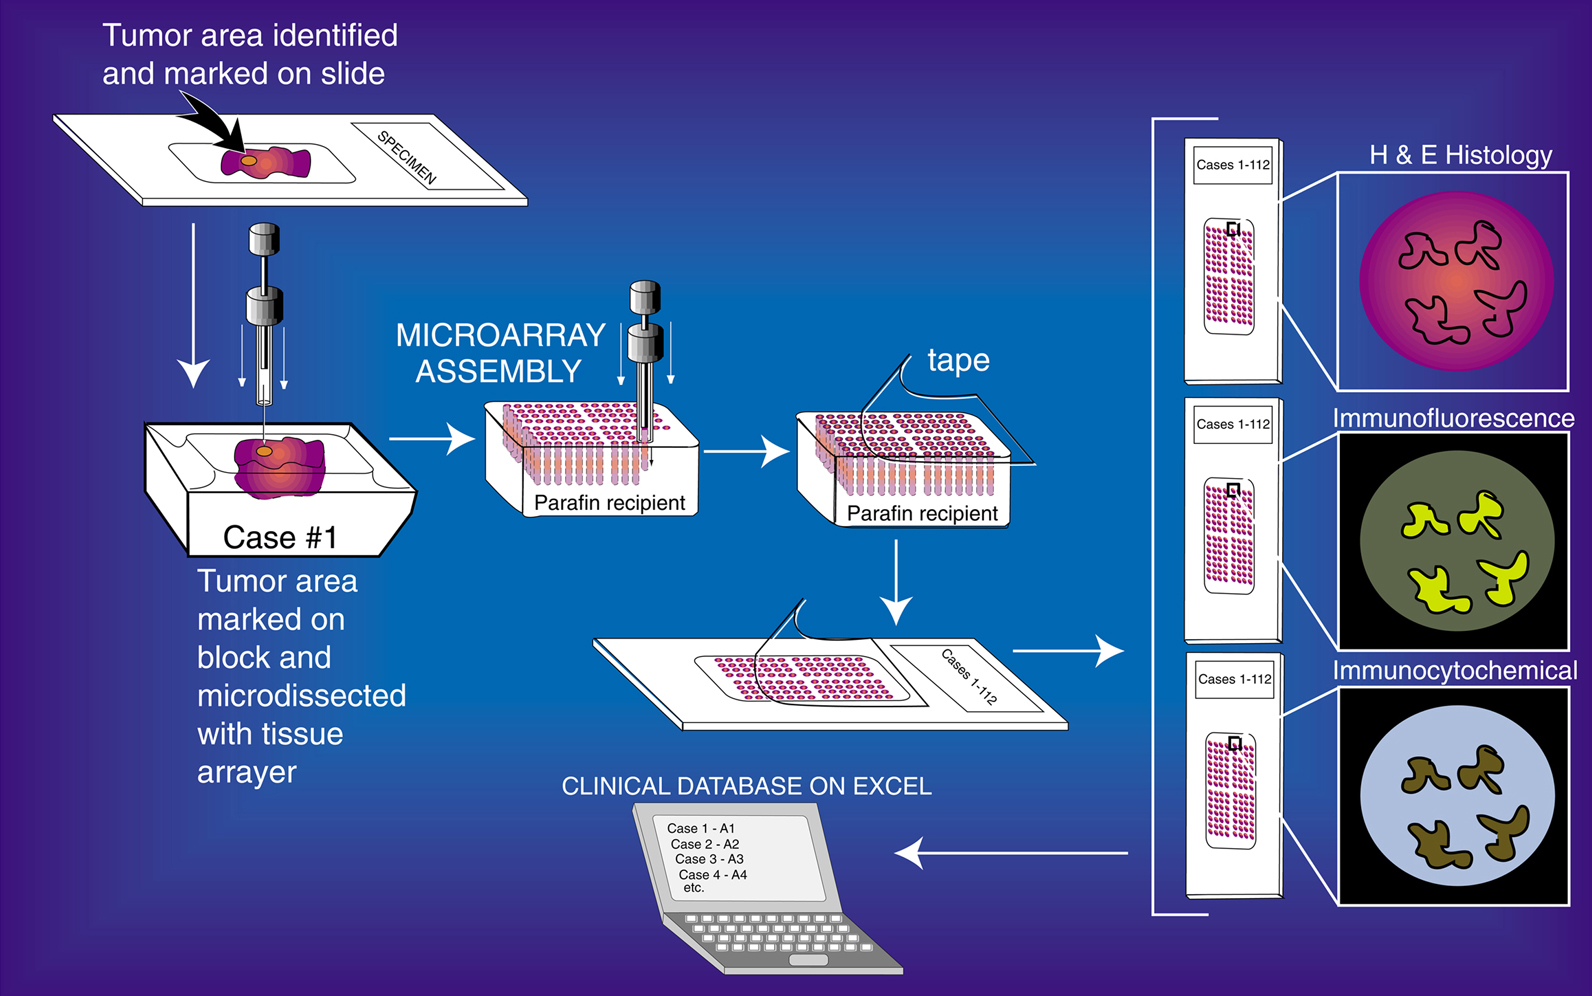
\includegraphics[width=4.5in]{/Users/ixc107/Documents/ICH_projects/CVetc/presentations/SI_Figures/Tissue_Microarray_Process.jpg}
		\end{figure} 
	}
	
	% % % % % % % % % % % % % % % % % % % % % % % % % % % % % % % % % % % % % slide 6

	\frame
	{\frametitle{Immunohistochemistry (IHC) in pathology}      
		\begin{itemize}
			\item Immunohistochemistry (IHC) refers to the process of selectively imaging antigens (e.g. proteins) in cells of a tissue section
			\item Traditionally, pathologists subjectively evaluate IHC marker levels based on staining intensity. This evaluation provides data in ordinal (e.g. low, medium and high) or nominal (positive/negative) scales.
			\item Machine-assisted image analysis platforms for IHC overcome the subjectivity of visual assessment and produce numeric data on the continuous scale.
		\end{itemize}
		\begin{figure}
	 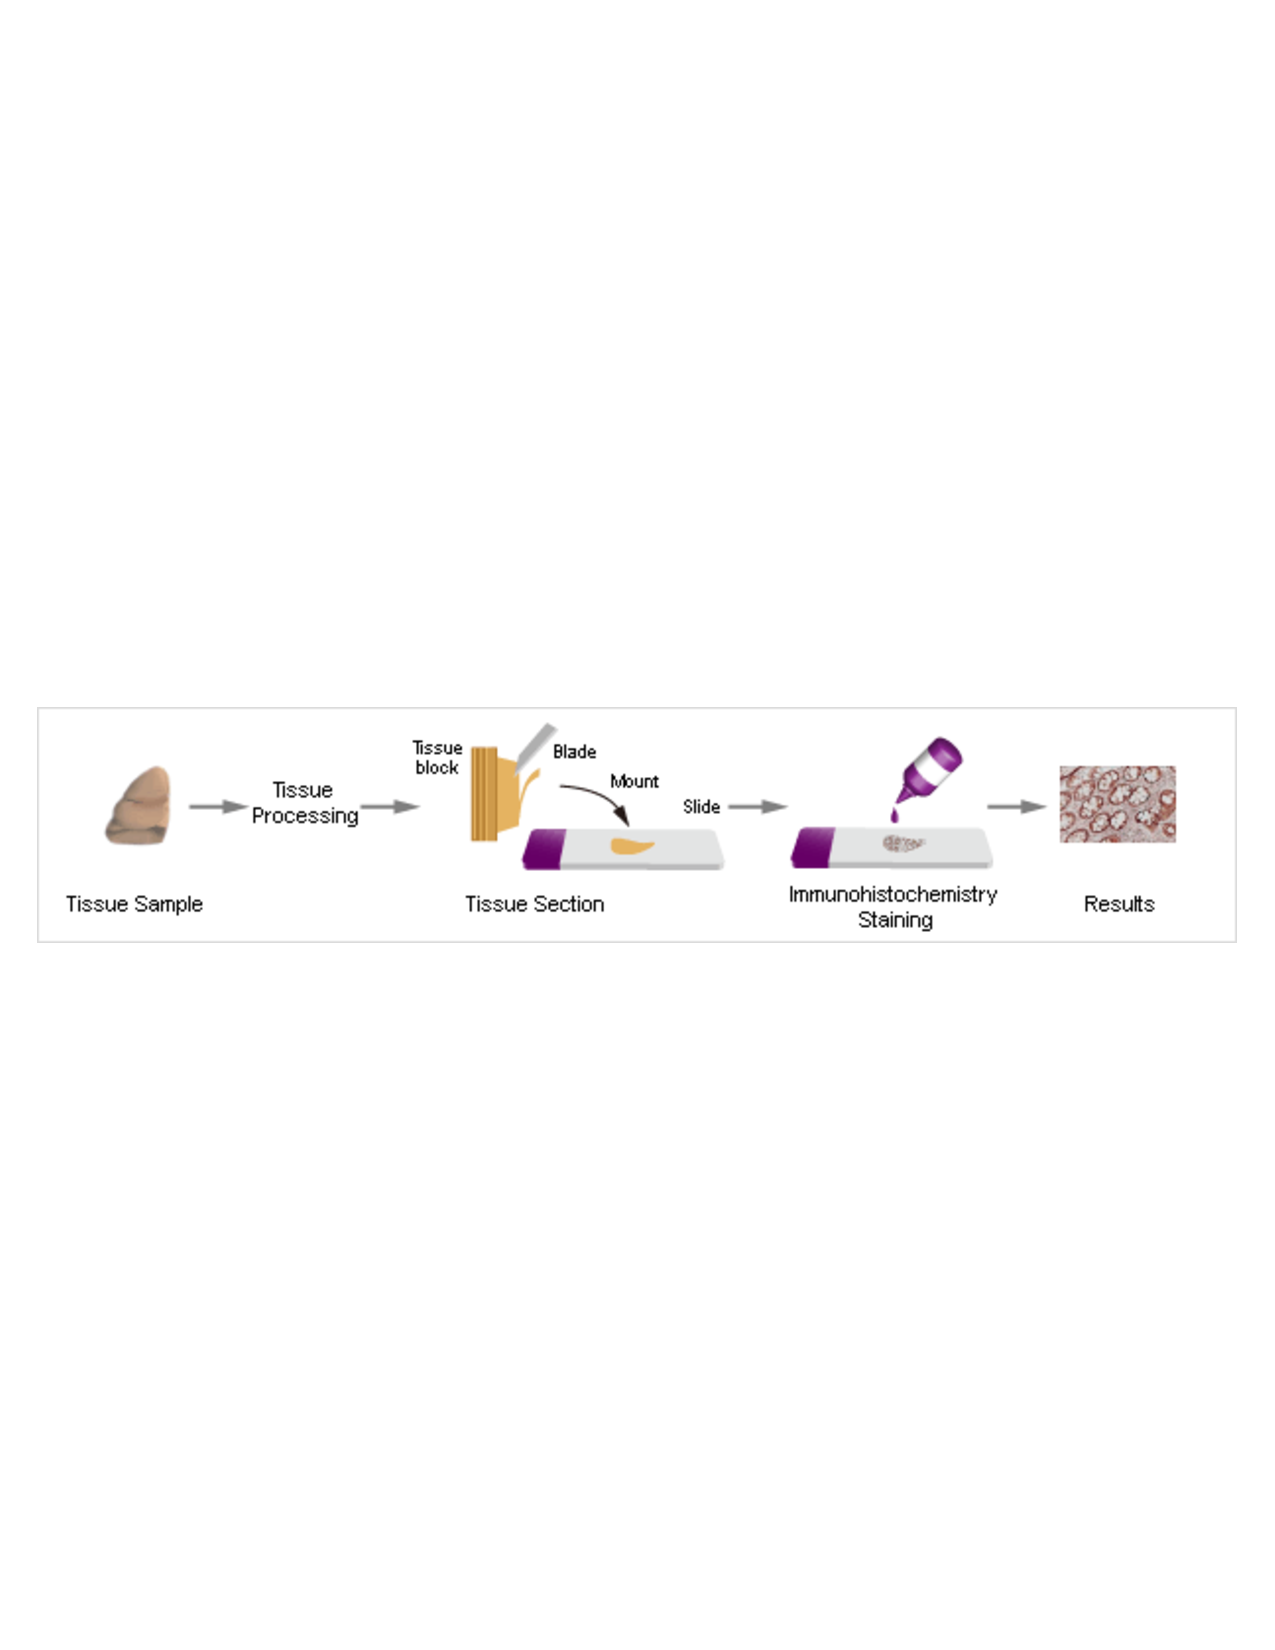
\includegraphics[width=4.5in] {/Users/ixc107/Documents/ICH_projects/CVetc/presentations/SIwebinarPhilaChapter/Figures/IHC_Service6.pdf}
			%	\includegraphics[width=4.5in] {"C:/Users/Misung Yi/Desktop/IBC2020/Figures/IHC_Service6".pdf}
		\end{figure} 
	}

	% % % % % % % % % % % % % % % % % % % % % % % % % % % % % % % % % % % % %  begin slide 7
	\frame
	{\frametitle{Immunofluorescence  IHC}   
		Immunofluorescence (IF) is a detection method, during which antibody binding to an antigen is visualized using a fluorophore. \\ Immunohistochemistry (IHC) refers to the process of selectively imaging antigens (e.g. proteins) in cells of a tissue section
		\begin{figure}
			\includegraphics[width=1.7in]{"C:/Users/Misung Yi/Desktop/IBC2020/Figures/Fig21_1".png}
			\caption{One tissue core image processed by Tissue Studio.
				
				\textbf{A}: Marker of interest produces pink colored signal, cell nuclei are colored in blue (DAPI), green colored are cancer cells (cytokeratin); %\textbf{B}: cancer region-of-interest is colored in red.
			} 
		\end{figure} 
	}
	
		% % % % % % % % % % % % % % % % % % % % % % % % % % % % % % % % % % % % %  begin slide 8
	\frame
	{\frametitle{Quantification of protein expression in IHC images}   
		\begin{itemize}
			\item  Integrated scanning and image analysis systems for pathology, e.g. \cite{Garcia-Rojo} enable measurement of proteins in individual cancer cells and their subcellular compartments, such as nuclei, cytoplasm or membranes.   
			\item  The standard IHC approach: \textbf{Mean Signal Intensity (MSI)} is computed within the region of interest (i.e. cancer cell compartment of the tumor).
			\item Advanced IHC software platforms detect the fluorescence signal in each pixel of the image, and then averaged over each compartment of interest (e.g. nucleus or cytoplasm of \textbf{every cancer cell}).
			\item The resulting entire distributions of  \textbf{cellular signal intensity (CSI)} of protein expression are available but usually ignored for analysis.  
			\item Only the MSI is usually considered as a biomarker ignoring the issue of heterogeneity in CSI signals.
  \color{red}
			\item However, for protein biomarkers that are heterogeneously expressed, it is not averaged levels, but rather low or high CSI levels that hold the greatest predictive power for clinical outcome.
			\color{black}
		\end{itemize}
	}


	% % % % % % % % % % % % % % % % % % % % % % % % % % % % % % % % % % % % %  begin slide 9
	\frame
	{\frametitle{Phosphorylated Stat5 (pYStat5) in breast cancer}   
		\begin{itemize}
			\item Representative IF IHC images of normal human breast tissue and two primary breast cancers 
			\item  pYStat5 (red, bottom), cytokeratin (green), and DNA (blue).
                \item pYStat5 is a latent cytoplasmic transcription factor and a primary mediator of prolactin signaling in breast epithelia.
  		\end{itemize}              
	 \begin{figure}
                \includegraphics[width=4.5in] {/Users/ixc107/Documents/ICH_projects/grants/R01_ICH/QImethods/FRQIdata/Tran_pYStat5fig.pdf}
	\end{figure} 
	}
	
		% % % % % % % % % % % % % % % % % % % % % % % % % % % % % % % % % % % % % slide 10
	\frame
	{\frametitle{Sample distributions of pYStat5 CSI signals}   
		\begin{figure}
                \includegraphics[width=4.5in] {/Users/ixc107/Documents/ICH_projects/grants/R01_ICH/presentations/JSM2021/mock_Density_fig.pdf}
     	\caption{           
    The same MSI levels (black vertical lines) may correspond to different CSI distributions. 
    Blue lines show the kernel density estimates for the distributions of Log CSI levels.}
		\end{figure} 
	}

%method 3-4 slides
	% % % % % % % % % % % % % % % % % % % % % % % % % % % % % % % % % % % % % begin slide  11
	
	\frame
	{\frametitle{Distributional approach to develop IHC protein biomarkers}	
			\begin{itemize}		
	\item  For each tissue sample of CSI expressions $\{x_{i},1\le i \le n\}$  and probability $p$, $0<p<1$, the
empirical quantile function $Q_{n}(p)$ is defined as the $j^{th}$ order statistic of the sample, where $j$ is such that $(j-1)/n<p<j/n$. 
     \item For $p=0.01,\dots, 0.99$ and $j=100×p$, $Q_{n}(p)$ is also known as $j^{th}$ percentile. 
     \item The empirical quantile function $Q_{n}(p)$ is an estimate of the theoretical (true) quantile function $Q(p)$, which is the inverse of the distribution function $F(x)$, that is $Q(F(x))=x$. 
     \item The advantage of using $Q_{n}(p)$, rather than more familiar empirical distribution function $F_{n}(p)$, is that $Q_{n}(p)$ is always defined on the interval [0,1] and can be analyzed in the framework of functional data analysis without "warping” (curve registration).
	\end{itemize}
		}
	% % % % % % % % % % % % % % % % % % % % % % % % % % % % % % % % % % % % % begin slide  12	
	
	\frame
	{\frametitle{Functional Regression Quantile Index (FR-QI)}
		\begin{itemize}		
		\item 
 For $k^{th}$ subject with the empirical quantile function $Q_{k}(p)$ of CSI expressions, FR-QI is defined as the functional regression predictor of outcome,
		 %an integral of subject's empirical quantile function $Q_{k}(p)$ multiplied by the coefficient function $\beta(p)$, 
		 \begin{center}
		 	$QI_{k}=QI_{k}(Q_{k}(p))= \int_{0}^{1} \beta(p)Q_{k}(p)dp$
		\end{center}
		\linebreak
		where $\beta(p)$ is an unknown functional coefficient function.
\item $\beta(p)$ represented either by a spline \cite{Ramsay2006} or by a piece-wise linear function \cite{James09} and estimated as part of fitting a model to a data set that includes clinical outcomes. 
	\item For continuous or dichotomous outcomes, $\beta(p)$ may be estimated using the R package \texttt{refund}.
	\item For survival outcomes, we propose to estimate $\beta(p)$ using the linear functional proportional hazards model \cite{Gellar15}, \cite{Cui20}
              \begin{center}
		 	$log h_{k}(t, \beta())=log h_{0} (t)+ \int_{0}^{1} \beta(p)Q_{k}(p)dp$
	    \end{center}
where $h_{k}[t,\beta()]$ is the hazard function at time $t$ and $h0(t)$ is a non-parametric baseline hazard function.	    
		\end{itemize}
	}		
		
	
		% % % % % % % % % % % % % % % % % % % % % % % % % % % % % % % % % % % % % begin slide  13
	\frame
	{\frametitle{Computation of pYStat5 FR-QI biomarker}
		\begin{itemize}	
			\item	Here the plots of quantile functions, estimated $\beta(p)$, and their products
		\end{itemize}
	}	
	
			% % % % % % % % % % % % % % % % % % % % % % % % % % % % % % % % % % % % % begin slide  14
		\frame
	{\frametitle{pYStat5 FR-QI vs. sample quantiles}
		\begin{itemize}	
			\item	Here the plots of pYStat5 FR-QI vs. sample quantile
		\end{itemize}
	}	

	% % % % % % % % % % % % % % % % % % % % % % % % % % % % % % % % % % % % % begin slide  15
	
	\frame
	{\frametitle{Dichotomization of FR-QI with internal validation}
		\begin{itemize}	
		      \item For clinical applications, it is often desired to use dichotomized FR-QI 
		      \item Dichotomization of FR-QI markers is implemented using the survival trees (recursive partitioning with 10-fold cross-validation, R package rpart)
			\item Internal validation of dichotomized FR-QI is conducted using the bootstrap optimism correction \cite{Steyerberg19}
			\item The optimism is defined as the decrease in performance between performance in the bootstrap sample and performance in the original sample 
			\bigskip
			\item Mean optimism estimate is calculated as the average optimism over 200-500 bootstrap samples
			\bigskip
			\item Optimism-corrected performance estimate is obtained by subtracting the mean optimism estimate from the estimate from original sample
		\end{itemize}
	}

		% % % % % % % % % % % % % % % % % % % % % % % % % % % % % % % % % % % % % begin slide  13
			
	\frame
	{\frametitle{Dichotomized pYStat5 FR-QI as predictor of PFS}
		\begin{itemize}	
			\item Table reporting results of Cox model and KM plot
		\end{itemize}
	}	

	% % % % % % % % % % % % % % % % % % % % % % % % % % % % % % % % % % % % % begin slide  17
	\frame
	{\frametitle{Conclusions}
		\begin{itemize}	
\item	 We developed a new framework for discovery of novel biomarkers based on cell level IHC data
\item	 The proposed FR-QI take into account tumor heterogeneity and entire distributions of CSI levels in a tumor sample.
\item	 FR-QI biomarkers are designed to adaptively up-weight the parts of CSI distributions most important for predicting clinical outcome
\item	 For pYStat5 CSI distributions, negative and increasing values of $\beta(p)$ imply that lower CSI levels correspond to higher FR-QI values and the highest magnitude of weights is in the range of lower percentiles.  This is consistent with previous findings that low Stat5 expression is associated with poor prognosis.
\item	 Meanwhile the standard pYStat5 mean signal intensity was not a predictor of PFS in our cohort of ER+ breast cancer patients
\item	 Thus, the proposed FR-QI may provide novel IHC biomarkers for proteins that do not have a prognostic value if only the mean signal intensity is considered.
  \end{itemize}
	}				


	% % % % % % % % % % % % % % % % % % % % % % % % % % % % % % % % % % % % % 
	% % % % % % % % % % % % % % % % % % % % % % % % % % % % % % % % % % % % % 
	% % % % % % % % % % % % % % % % % % % % % % % % % % % % % % % % % % % % % 
	% % % % % % % % % % % % % % % % % % % % % % % % % % % % % % % % % % % % % 
	% % % % % % % % % % % % % % % % % % % % % % % % % % % % % % % % % % % % % 
	% % % % % % % % % % % % % % % % % % % % % % % % % % % % % % % % % % % % % 
	% % % % % % % % % % % % % % % % % % % % % % % % % % % % % % % % % % % % % 
	
	\begin{comment}

	% % % % % % % % % % % % % % % % % % % % % % % % % % % % % % % % % % % % % begin slide  9

	\frame
	{\frametitle {Marked point processes approach}  
		\begin{itemize} 
		\color{red}
		\item We consider the patterns of spatial localization of protein expression levels in cells or their nuclei (CSI signals) for developing novel IHC biomarkers. 
		\color{black}
		\item The methods are developed in the framework of the \textbf{marked point processes}
		\item The point patterns of nuclei or cells centroids in the tumor tissue are viewed as realizations of a \textbf{point process}. 
		\item A spatial \textbf{point process} is a random pattern of points, both the number of points and their locations being random.
		\item A \textbf{marked point processes} is a point process combined with some associated quantities (`marks') measured at each point.
		\item We view protein expression CSI levels as  \textbf{marks} in a marked point process of cancer cells/nuclei centroids in the tissue.
		\item Point pattern of cells centroids of cancer cells + CSI levels of protein expression $=>$ \textbf{marked point pattern (MPP)}
		\item An \textit{independently marked} point process has marks that are independent, identically distributed and independent of the locations.
	\end{itemize}  
}
	% % % % % % % % % % % % % % % % % % % % % % % % % % % % % % % % % % % % %    
	\frame
	{\frametitle{Example 1 of a marked point pattern of Ki67}   
		\begin{columns}
			\column{0.55\textwidth}
			\includegraphics[height=2in]{"C:/Users/Misung Yi/Desktop/IBC2020/Figures/Ki67/mpp_AAMCaB03".pdf}
			\column{0.55\textwidth}
			\includegraphics[height=2in] {"C:/Users/Misung Yi/Desktop/IBC2020/Figures/Ki67/AAMCa-B03_10X_Ki67_HiEMark".pdf}
		\end{columns}
		In MPP, the centers of the plotting circles in are at the cancer cell centroids, the radii of the plotting circles are proportional to the Ki67 expression. The left panel shows the CSI levels corresponding to the radii of the plotting circles.
	}
	
	% % % % % % % % % % % % % % % % % % % % % % % % % % % % % % % % % % % % %    
	\frame
	{\frametitle{Example 2 of marked point pattern of Ki67}   
		\begin{columns}
			\column{0.6\textwidth}
			\includegraphics[height=2in]{"C:/Users/Misung Yi/Desktop/IBC2020/Figures/Ki67/mpp_TJUe_G17".pdf}
			\column{0.6\textwidth}
			\includegraphics[height=2in] {"C:/Users/Misung Yi/Desktop/IBC2020/Figures/Ki67/TJUe_G17_12x_Ki67".pdf}
		\end{columns}
	}
	
	% % % % % % % % % % % % % % % % % % % % % % % % % % % % % % % % % % % % % begin slide 17   
	\frame
	{\frametitle {Conditional Mean and Variance of marks in MPP}  
		\begin{itemize} 
			\item   
			Denote by $\Psi = \cup_{i} \{ ( \mathbf{u}_{i}, m(\mathbf{u}_{i}) ),  \mathbf{u}_{i} \in P \}$, a marked point process with a real-valued mark function $m(\mathbf{u}_{i})$ defined at each point $\mathbf{u}_{i}$.
			
			\item Conditional mean $cMean(d)$ and conditional variance $cVar(d)$ of a mark given that there is another point of the process a distance $d$ away \cite{Schlather04} are defined as:
			
			\begin{center}
				$cMean(d)=E[m(\mathbf{u}) \vert \mathbf{u},  \mathbf{v} \in P, \left\Vert \mathbf{u}-\mathbf{v}\right\Vert =d ]$ 
			\end{center}
			
			\begin{center}
				$cVar(d)=E [ \{m(\mathbf{u}) - cMean(d) \}^{2} \vert \mathbf{u},  \mathbf{v} \in P, \left\Vert \mathbf{u}-\mathbf{v}\right\Vert =d ]$ 
			\end{center}
			
			\item That is, $cMean(d)$ and $cVar(d)$ are \textbf{\textit{functions}} of the distance $d$ between points $\mathbf{u}, \mathbf{v} \in
			P$. But if marks and points are independent, $cMean(d)$ and $cVar(d)$ are constant functions of the inter-point distance $d$.
			\color{red}
			\item \textbf{ $cMean(d)$ and $cVar(d)$ are the standard mean and variance of the marginal distribution of marks if marks and points are independent.}
			\color{black}
			\item In this work, $cMean(d)$ and $cVar(d)$ are estimated using nonparametric kernel density estimator under the assumption of \emph{second-order intensity reweighted stationary processes} \cite{Baddeley00} \\
			(Implemented in R package \texttt{spatstat} \cite{Baddeley05}).
		\end{itemize}  
	}
	
	% % % % % % % % % % % % % % % % % % % % % % % % % % % % % % % % 

	\frame
	{\frametitle {Estimation of $cMean(d)$ and $cVar(d)$ }  
		\begin{itemize} 
			
			\item  Nonparametric estimates of $cMean(d)$ and $cVar(d)$ \cite{Schlather04}:
			
			\begin{center}
				$\widehat{cMean}\left( d\right)
				=N_{d}^{-1}\sum\limits_{\left\vert \left\Vert \mathbf{u}_{k}-\mathbf{u}%
					_{l}\right\Vert -d\right\vert \leq \varepsilon /2}m\left( \mathbf{u}_{k}\right),$
			\end{center} 
			
			\begin{center}
				$\widehat{cVar}\left( d\right) =N_{r}^{-1}\sum\limits_{\left\vert \left\Vert 
					\mathbf{u}_{k}-\mathbf{u}_{l}\right\Vert -d\right\vert \leq \varepsilon /2}%
				\left[ m\left( \mathbf{u}_{k}\right) -\widehat{cMean(d)}\right]
				^{2},$ 
			\end{center}
			\noindent where $d\geq 0,$ is a distance between two points, $\varepsilon >0$ is a fixed bin width and $N_{d}$ is
			the number of pairs $\left( \mathbf{u}_{k},\mathbf{u}_{l}\right)$ such that
			$\left\vert \left\Vert \mathbf{u}_{k}-\mathbf{u}_{l}\right\Vert
			-d\right\vert \leq \varepsilon /2$. 
			
			\item In this work, $cMean(d)$ and $cVar(d)$ are estimated using nonparametric kernel density estimator under the assumption of \emph{second-order intensity reweighted stationary processes} \cite{Baddeley00} \\
			(Implemented in R package \texttt{spatstat} \cite{Baddeley05}).
		\end{itemize}  
	}

	% % % % % % % % % % % % % % % % % % % % % % % % % % % % % % % %  begin slide 18   
	
	\frame
	{\frametitle {Ki67 MPPs and estimators of cMean and cVar}  
		\begin{figure}
			\part{\part{title}}\includegraphics[height=3in] {"C:/Users/Misung Yi/Desktop/IBC2020/Figures/Ki67show".pdf}
		\end{figure} 
	}
	
	% % % % % % % % % % % % % % % % % % % % % % % % % % % % % % % % % % % % % begin slide 19   
	\frame
	{\frametitle {Spatial Indices based on $cMean(d)$ and $cVar(d)$}  
		
		\begin{itemize} 
			
			\item  For the $i^{th}$ tissue MPP, let $\widehat{cMean}\left( d\right)$ and $\widehat{cVar}\left( d\right)$ be the kernel density estimates of $cMean_{i}(d)$ and $cVar_{i}(d)$, respectively.  
			\item  We consider the following spatial indices (SIs):
			\begin{center}
				\noindent  $AUcMean_{i}\left( d_{max}\right)=d_{max}^{-1}\int_{0}^{d_{max}} \widehat{cMean_{i}}\left( r\right)dr$
			\end{center}
			\begin{center}
				\noindent   $AUcVar_{i}\left( d_{max}\right)=d_{max}^{-1}\int_{0}^{d_{max}} \widehat{cVar_{i}}\left( r\right)dr$
			\end{center}
			where $d_{max}$ is optimized using the standard training and validation strategy.  
			\item In this work, $AUcMean(d_{max})$ and $AUcVar( d_{max})$ were computed for $d_{max}=12,13,\dots,100$ ($6\mu m$ is the
			median diameter of the cancer cells and $100\mu m$ is the average size of clusters of cancer cells).
			\item Survival tree model (R package \texttt{rpart}) was used to establish optimal cutoff for dichotomizing $AUcMean_{i}\left( d_{max}\right)$ and $AUcVar_{i}\left( d_{max}\right)$ in the training set. 
			\item Optimal $d^{M}_{max}$ and $d^{V}_{max}$ were selected corresponding to the largest effect size for dichotomized $AUcMean_{i}\left( d_{max}\right)$ and $AUcVar_{i}\left( d_{max}\right)$ in the validation set. 
			\item  Dichotomized $AUcMean\left( d^{M}_{max}\right)$ and $AUcVar\left( d^{V}_{max}\right)$ were evaluated in the test set (Kaplan-Meier survival curves and Cox proportional hazards models).
		\end{itemize} 
	}
	
	% % % % % % % % % % % % % % % % % % % % % % % % % % % % % % % % % % % % %  Ki67  results
	
	\frame
	{\frametitle{Analysis results for Ki67 markers in the test set}  
		Optimal $d^{M}_{max}=30\mu m$ and $d^{V}_{max}=78\mu m$ were selected in the validation phase.   
		\begin{figure}
			\begin{center}
				\begin{columns}
					\column{0.3\textwidth}
					\includegraphics[height=1.3in]{"C:/Users/Misung Yi/Desktop/IBC2020/Figures/Ki67/results/Fig2A1".pdf}
					\includegraphics[height=1.4in]{"C:/Users/Misung Yi/Desktop/IBC2020/Figures/Ki67/results/FigMSI".pdf}
					\column{0.3\textwidth}
					\includegraphics[height=1.3in]{"C:/Users/Misung Yi/Desktop/IBC2020/Figures/Ki67/results/Fig2A2".pdf}
					\includegraphics[height=1.4in]{"C:/Users/Misung Yi/Desktop/IBC2020/Figures/Ki67/results/Fig2a_cMean".pdf}
					\column{0.3\textwidth}
					\includegraphics[height=1.3in]{"C:/Users/Misung Yi/Desktop/IBC2020/Figures/Ki67/results/Fig2A3".pdf}
					\includegraphics[height=1.4in]{"C:/Users/Misung Yi/Desktop/IBC2020/Figures/Ki67/results/Fig2a_cVar".pdf}
				\end{columns}
			\end{center}
		\end{figure} 
	}
	
	% % % % % % % % % % % % % % % % % % % % % % % % % % % % % % % % % % % % %   
	
	\frame
	{\frametitle{Analysis results for Ki67 markers in the test set (cont)}  
		\begin{figure}
			\begin{center}
				\begin{columns}
					\column{0.3\textwidth}
					\includegraphics[height=1.7in]{"C:/Users/Misung Yi/Desktop/IBC2020/Figures/Ki67/results/Fig2B".pdf}
					\column{0.7\textwidth}
					\includegraphics[height=1.7in]{"C:/Users/Misung Yi/Desktop/IBC2020/Figures/TableKi67".pdf}
				\end{columns}
			\end{center}
		\end{figure} 
		Dichotomized Ki67 MSI yielded HR=1.79 (95\%CI: 1.06-3.05; p=0.034) in the multivariable Cox model with the same clinico-pathological prognostic factors. 
	}
	
	% % % % % % % % % % % % % % % % % % % % % % % % % % % % % % % % % % % % %   
	

	
	\frame
	{\frametitle{Simulation of MPPs}  
		\begin{itemize} 
			\item Three different types of MPPs were simulated in ($[0,1]\times[0,1]$).
			\item  \textbf{Type A: ``Nearly Homogeneous"} MPPs simulated with points as realizations of the uniform Poisson process with intensity 100 ($Poisson(100)$) and log-transformed marks $\sim N(3.8, 0.5^{2})$. 
			
			\item \textbf{Type B: ``Salt-and-pepper mixture"} MPPs simulated as superimposed mixtures of two independent marked point processes, $Poisson(80)$ with log(marks)$\sim N(3.0, 0.5^{2})$ and $Poisson(20)$ with log(marks)$\sim N(5.0, 0.5^{2})$.
			
			\item \textbf{Type C: ``High-signal clustered"} MPPs simulated as superimposed mixtures of independent $Poisson(80)$ with log(marks)$\sim N(2.25, 0.3^{2})$ and Matern clustered point process with log(marks)$\sim N(5.0, 0.5^{2})$.
			
			\item For \textbf{Type C1} MPPs, the Matern clustered point process had intensity 10 for the Poisson process of cluster centers, 0.1 as the radius parameter of the clusters, and 3 as the mean number of points per cluster. 
			
			\item For \textbf{Type C2} MPPs, the Matern clustered point process had intensity 2 for the Poisson process of cluster centers,  0.2 as the radius parameter of the clusters, and 15 as the mean number of points per cluster. 
			
		\end{itemize} 
	}
	% % % % % % % % % % % % % % % % % % % % % % % % % % % % % % % % % % % % %  
	\frame
	{\frametitle{Examples of simulated MPPs}                 
		\begin{columns}
			\column{0.25\textwidth}
			\begin{center}
				\textbf{Type A}      
				\includegraphics[height=1.2in]{"C:/Users/Misung Yi/Desktop/IBC2020/Figures/SimFigs/Fig5_A".pdf}
				\includegraphics[height=1.2in]{"C:/Users/Misung Yi/Desktop/IBC2020/Figures/SimFigs/Fig5cEcV_A".pdf}     
			\end{center}
			\column{0.25\textwidth}
			\begin{center}
				\textbf{Type B}       
				\includegraphics[height=1.2in]{"C:/Users/Misung Yi/Desktop/IBC2020/Figures/SimFigs/Fig5_B".pdf}
				\includegraphics[height=1.2in]{"C:/Users/Misung Yi/Desktop/IBC2020/Figures/SimFigs/Fig5cEcV_B".pdf}         
			\end{center}
			\column{0.25\textwidth}
			\begin{center}
				\textbf{Type C1}   
				\includegraphics[height=1.2in]{"C:/Users/Misung Yi/Desktop/IBC2020/Figures/SimFigs/Fig5_C".pdf}
				\includegraphics[height=1.2in]{"C:/Users/Misung Yi/Desktop/IBC2020/Figures/SimFigs/Fig5cEcV_C".pdf}         
			\end{center}
			\column{0.25\textwidth}
			\begin{center}
				\textbf{Type C2}   
				\includegraphics[height=1.2in]{"C:/Users/Misung Yi/Desktop/IBC2020/Figures/SimFigs/Fig5_D".pdf}
				\includegraphics[height=1.2in]{"C:/Users/Misung Yi/Desktop/IBC2020/Figures/SimFigs/Fig5cEcV_D".pdf}       
			\end{center}  
		\end{columns}
	}
	
	% % % % % % % % % % % % % % % % % % % % % % % % % % % % % % % % % % % % %  
	\frame
	{\frametitle{$AUcMean$ vs. $AUcVar$ vs. MSI by simulated MPP type} 
		\begin{center}   
			\includegraphics[height=0.95in]{"C:/Users/Misung Yi/Desktop/IBC2020/Figures/SimFigs/Fig5_I".pdf} 
			\includegraphics[height=0.95in]{"C:/Users/Misung Yi/Desktop/IBC2020/Figures/SimFigs/Fig5_K".pdf}          
			\includegraphics[height=0.95in]{"C:/Users/Misung Yi/Desktop/IBC2020/Figures/SimFigs/Fig5_L".pdf}    
		\end{center}  
	}   

	% % % % % % % % % % % % % % % % % % % % % % % % % % % % % % % % % % % % %
	\frame
	{\frametitle {Simulation study of MPP type predicting surival outcome}  
		\begin{itemize} 
			\item Survival outcomes were generated using the R package \texttt{survsim} \cite{Morina} under assumptions of Weibull distributions for time to event and time to censoring.
			\item Event rates were similar to the recurrence rates in breast cancer TMA data.
			\item Each training and test data set included 60, 90 or 120 subjects per risk group. 
			\item Simulated datasets were binned with similar hazard ratios (HR) in intervals [1.5-2.0], [2.0-2.5], $\dots$, [4.5-5.0], [5.0-6.0].
			\item  Different MPP types were associated with different risk groups (high vs. low).  
			\item The training set was used to identify cutoffs for MSI, $AUcMean\left( d_{max}\right)$ and $AUcVar\left( d_{max}\right)$ for  $d_{max}=0.2$ using survival tree models.
			\item  The optimal cutoff was then used to predict high and how risk groups in the test set and resulting prediction was compared to the risk group simulated. 
			\item  The misclassification error (MCE) was computed as a proportion of subjects with incorrectly predicted risk groups in each test set matched with the training set that yielded a cutoff for dichotomization.
			
		\end{itemize}  
	}
	
	% % % % % % % % % % % % % % % % % % % % % % % % % % % % % % % % % % % % %  
	\frame
	{\frametitle{Results predicting risk groups with different MPP types} 
		\begin{center}   
			\includegraphics[width=4.8in]{"C:/Users/Misung Yi/Desktop/IBC2020/Figures/SimFigs/Fig5_M".pdf}          
			\includegraphics[width=4.8in]{"C:/Users/Misung Yi/Desktop/IBC2020/Figures/SimFigs/PropWOcutoff_same_rawMSIs".pdf}    
		\end{center} 
		Results are shown only for the simulated data sets with 90 subjects per risk group.  Results for other sample sizes (60 and 120 subjects) were very similar.
	}   

	% % % % % % % % % % % % % % % % % % % % % % % % % % % % % % % % % % % % %  concluding  
	\frame
	{\frametitle {Conclusions}  
		\begin{itemize} 
			\item  We developed a methodology that provides objective means to quantify intratumoral heterogeneity of proteins in IHC images at single cell resolution.
			\item The proposed spatial indices $AUcMean$ and $AUcVar$ provide numeric metrics that can discriminate between different common types of intra-tumoral heterogeneity of CSI levels.
			\item $AUcVar$ metric of CSI expression heterogeneity may provide prognostic information either when the standard MSI levels can serve as outcome predictors (Ki67 case)  
			\item $AUcVar$ provides an objective quantitative tool for detecting microclusters of high CSI levels that are not readily noticeable by visual image evaluation. 
			\item Previously considered spatial methods to study tumor heterogeneity are based on multi-type marked point process that require prior determination of expression category (by a pathologist).
			\item Our approach is directly applicable to any histology-based quantification method that allows capturing continuous expression levels in individual cells or cell compartments.
		\end{itemize}  
	}

	\end{comment}
	% % % % % % % % % % % % % % % % % % % % % % % % % % % % % % % % % % % % % 
	\frame
	{\frametitle { }  
		\vfill
		\begin{figure}
			\includegraphics[height=0.8in] {"C:/Users/Misung Yi/Desktop/IBC2020/Figures/Thank_you".pdf}
		\end{figure} 
		\vfill
	}
	
	% % % % % % % % % % % % % % % % % % % % % % % % % % % % % % % % % % % % %  begin slide 27   
	\frame
	{\frametitle {References}  
		
		\begin{thebibliography}{ }
			
			\bibitem[Garcia-Rojo, 2012] {Garcia-Rojo}
			Garcia-Rojo M. State of the art and trends for digital pathology. \textit{Studies in health technology and informatics}. 2012;179:15-28.
								
			\bibitem[Ramsay, 2006] {Ramsay2006}
			Ramsay, J. O. (2006). \textit{Functional data analysis}. John Wiley and Sons, Inc..
			
			\bibitem[James, 2002] {James02}
			James G. Generalized linear models with functional predictor variables. \textit{Journal of the Royal Statistical Society}. 2002; 64(Series B):411-32.
			
			\bibitem[James et al, 2009] {James09}
			James G, Wang, J., Zhu, J. Functional Linear Regression That's Interpretable. \textit{Annals of Statistics}. 2009;37:2083-108.
			
			\bibitem[Gellar et al, 2015] {Gellar15}
		Gellar, J. E., Colantuoni, E., Needham, D. M., and Crainiceanu, C. M. (2015), “CoxRegressionModelsWith FunctionalCovariates for Survival Data,\textit{Statistical Modelling}, 15, 256–278.
			
		\bibitem[Cui et al, 2020] {Cui20}
		Cui, E., Crainiceanu, C.M. and Leroux, A., 2020. Additive Functional Cox Model. Journal of Computational and Graphical Statistics, pp.1-14.
						
			\bibitem[Steyerberg, 2019] {Steyerberg19}
			Steyerberg, E. W. (2019). \textit{Clinical prediction models}.  Springer.
			
		\end{thebibliography}
	}

\begin{comment}

	% % % % % % % % % % % % % % % % % % % % % % % % % % % % % % % % % % % %  
	\frame
	{\frametitle {Intensity function of the point process}  
		\begin{itemize} 
			\item Let $P$ be a planar spatial point process in a bounded region $D\subset \boldsymbol{R}%
			^{2}$. 
			
			\bigskip
			\item Let $N_{P}(B)$\ be the count function of $P$, which is the number of
			points falling into any Borel set $B\subset D,$ and $\left\vert B\right\vert 
			$ be the Lebesque measure of $B.$ 
			
			\bigskip
			\item For $\mathbf{u}_{1},...\mathbf{u}_{k}\in
			P,$ the $k^{th}$ order \textbf{intensity function} is defined by 
			
			\bigskip
			$\lambda _{k}\left( 
			\mathbf{u}_{1},...,\mathbf{u}_{k}\right) =\mathbf{\lim_{\left\vert d\mathbf{u%
					}_{1}\right\vert \cdot \cdot \cdot \left\vert d\mathbf{u}_{k}\right\vert
					\rightarrow 0}}\left\{ \frac{E\left[ N\left( d\mathbf{u}_{1}\right) \cdot
				\cdot \cdot N\left( d\mathbf{u}_{k}\right) \right] }{\left\vert d\mathbf{u}%
				_{1}\right\vert \cdot \cdot \cdot \left\vert d\mathbf{u}_{k}\right\vert }%
			\right\} $,
			
			\bigskip
			where $d\mathbf{u}_{k}$ is an infinitesimal region which contains the point
			$\mathbf{u}_{k}$ 
			
			and $\left\vert d\mathbf{u}_{k}\right\vert$ is its volume.
			
		\end{itemize}  
	}
	
	% % % % % % % % % % % % % % % % % % % % % % % % % % % % % % % % % % % %  
	\frame
	{\frametitle {First order intensity of the point process}  
		\begin{itemize} 
			
			\item The first order intensity is
			$\lambda _{1}\left(\mathbf{u}_{1} \right) =\mathbf{\lim_{\left\vert d\mathbf{u%
					}_{1}\right\vert
					\rightarrow 0}}\left\{ \frac{E\left[ N\left( d\mathbf{u}_{1}\right) \right] }{\left\vert d\mathbf{u}%
				_{1}\right\vert }%
			\right\} $. 
			\item The first order intensity $\lambda _{1}\left(\mathbf{u}_{1} \right)$ represents the mean number of points per unit area centered at $\mathbf{u} $
			\item The point process $P$ is called \textbf{stationary} if $\lambda _{1}\left( \mathbf{u}\right) \equiv \lambda 
			$ (constant intensity or homogeneous process). 
			\item Statistical methods for analysis of the marked point processes usually assume either fully parametric models for intensity or homogeneous intensity of the point process (stationary marked point process).
			\color{red}
			\item  But the cancer cell nuclei point patterns are generally inhomogeneous.
			\color{black}
		\end{itemize}  
	}
	
	% % % % % % % % % % % % % % % % % % % % % % % % % % % % % % % % % % % %  
	\frame
	{\frametitle {Second order intensity of the point process}  
		\begin{itemize} 
			
			\item 
			For $\mathbf{u}_{1},\mathbf{u}_{2}\in
			P,$ the $\mathbf2^{nd}$ \textbf{order intensity function} is defined by 
			
			\bigskip
			$\lambda _{2}\left( 
			\mathbf{u}_{1},...,\mathbf{u}_{k}\right) =\mathbf{\lim_{\left\vert d\mathbf{u%
					}_{1}\right\vert , \left\vert d\mathbf{u}_{2}\right\vert
					\rightarrow 0}}\left\{ \frac{E\left[ N\left( d\mathbf{u}_{1}\right) , N\left( d\mathbf{u}_{2}\right) \right] }{\left\vert d\mathbf{u}%
				_{1}\right\vert \left\vert d\mathbf{u}_{k}\right\vert }%
			\right\} $. 
			
			\bigskip
			\item 
			$\lambda _{2}\left( \mathbf{u}_{1},...,\mathbf{u}_{k}\right)\left\vert d\mathbf{u}%
			_{1}\right\vert  \left\vert d\mathbf{u}_{k}\right\vert$  
			is the approximate probability that $\left\vert d\mathbf{u}%
			_{1}\right\vert$ and  $\left\vert d\mathbf{u}_{2}\right\vert$ each contains an
			event from $P$, where $\mathbf{u}_{1} \ne \mathbf{u}_{2}$.
			
			\bigskip
			\item 
			If $P$ is stationary, then 
			$\lambda _{2}\left(\mathbf{u}_{2},\mathbf{u}_{2}\right)=\lambda _{2}\left(\mathbf{0},\mathbf{u}_{1}-\mathbf{u}_{k}\right)$
			
			
		\end{itemize}  
	}
	
	% % % % % % % % % % % % % % % % % % % % % % % % % % % % % % % % % % % %  
	\frame
	{\frametitle {Second-order intensity reweighted stationary processes}  
		\begin{itemize} 
			\item  \textbf{Pair correlation function} is
			defined as 
			
			\bigskip
			$\rho \left( \mathbf{u},\mathbf{v}\right) =\lambda _{2}\left( 
			\mathbf{u},\mathbf{v}\right) \left[ \lambda _{1}\left( \mathbf{u}\right)
			\lambda _{1}\left( \mathbf{v}\right) \right] ^{-1}$,
			\bigskip 
			
			assuming that the intensity functions exist for $k\leq 2$ and the
			first order intensity $\lambda _{1}\left( \mathbf{u}\right) $ is strictly
			positive, but not necessarily constant.
			\bigskip 
			
			\item The pair correlation function $\rho
			\left( \mathbf{u},\mathbf{v}\right) $ is called \textbf{translation invariant} if 
			$\rho
			\left( \mathbf{u},\mathbf{v}\right) =\rho \left( \left\Vert \mathbf{u}-%
			\mathbf{v}\right\Vert \right)$,
			where $\left\Vert \mathbf{u}-\mathbf{v}%
			\right\Vert =r$ is a Euclidian norm and $\rho (r):\left[ 0,\infty \right)
			\rightarrow \left[ 0,\infty \right) $. 
			\bigskip 
			\item The point process $P$ is called the \textbf{ \textit{second-order intensity
					reweighted stationary}}  if $\rho
			\left( \mathbf{u},\mathbf{v}\right) $ is translation invariant [Baddeley et al, 2000].
			\bigskip 
			\item The second-order intensity reweighted stationary processes allow accommodating marked point processes with \emph{variably inhomogeneous} point patterns of cancer cells or nuclei.
		\end{itemize}  
	}
	
	\end{comment}
	
	
\end{document}






